\section{Theory of Operations}

The SPI (Serial Peripheral Interface) core is equipped with a variety of features that make it a versatile and efficient choice for synchronous serial communication in embedded systems. Below is a detailed list of its key features:

\begin{itemize}
    \item \textbf{Full Duplex, Three-Wire Synchronous Data Transfer:} Enables simultaneous transmission and reception of data, enhancing communication efficiency.
    \item \textbf{Master or Slave Operation:} The SPI core can function as either a master, initiating and controlling communication, or as a slave, responding to the master's commands.
    \item \textbf{LSb First or MSb First Data Transfer:} Flexibly configures the data transmission order based on the system requirements, supporting both Least Significant Bit (LSb) first and Most Significant Bit (MSb) first formats.
    \item \textbf{Programmable Bit Rates:} Allows customization of the SPI clock speed to match the performance needs of different peripherals and system constraints.
    \item \textbf{End of Transmission Interrupt Flag:} Notifies the system when a data transmission cycle is complete, facilitating efficient interrupt-driven communication.
    \item \textbf{Write Collision Protection:} Prevents data corruption by detecting and handling scenarios where multiple write attempts occur simultaneously.
    \item \textbf{Wake-up from Idle Mode:} Supports low-power operations by enabling the SPI core to wake up from idle states upon specific events or triggers.
    \item \textbf{Double-Speed Master SPI Mode:} Increases data throughput by doubling the SPI clock rate in master mode, enhancing overall system performance.
\end{itemize}

% Block Diagram
\begin{figure}[H]
    \centering
    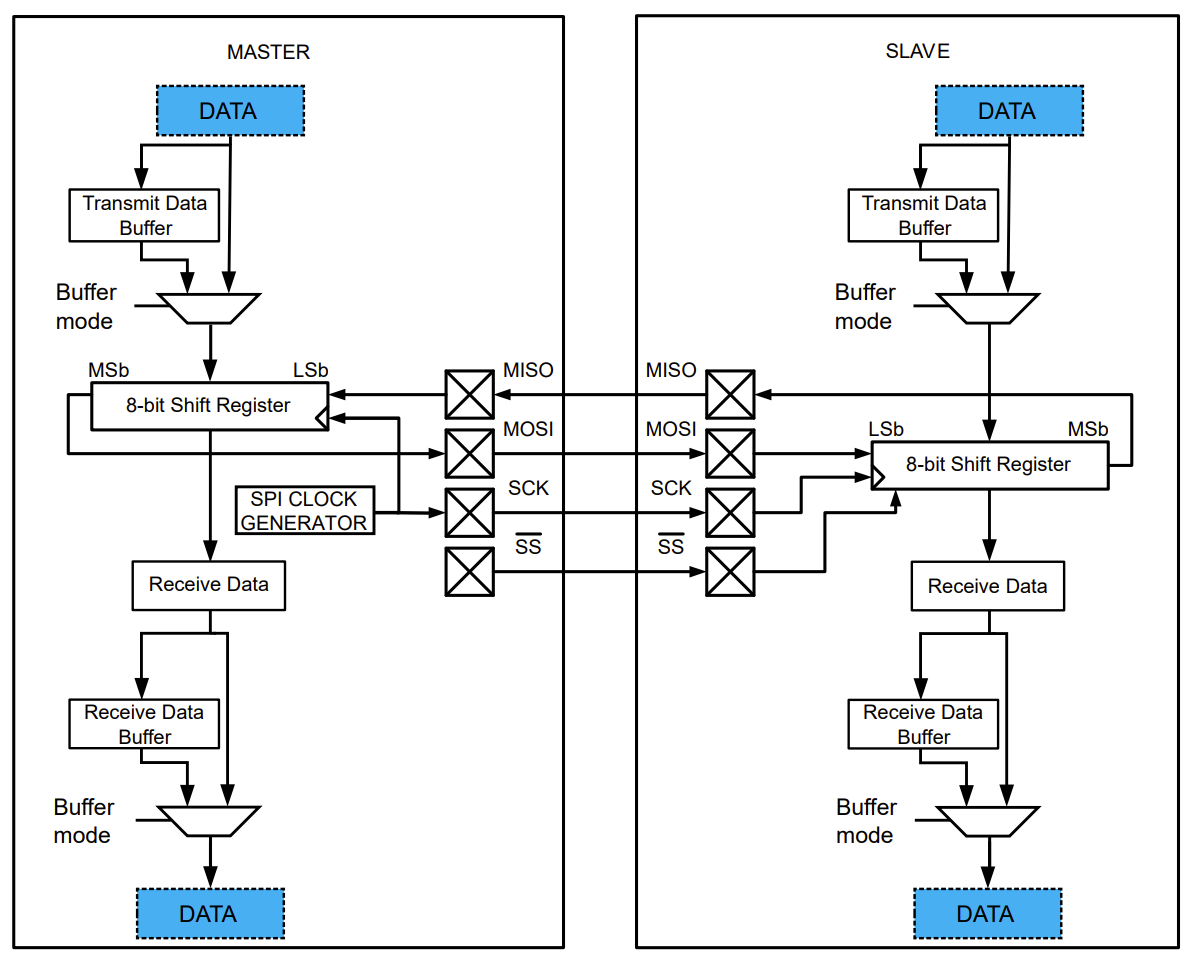
\includegraphics[width=0.8\textwidth]{images/spi_block_diagram.png}
    \caption{SPI Core Block Diagram}
    \label{fig:spi_block_diagram}
\end{figure}

\subsection{Overview}
The Serial Peripheral Interface (SPI) core is a robust and high-speed synchronous communication protocol widely used in embedded systems. It facilitates reliable data exchange between a central controller (master) and various peripheral devices (slaves) such as sensors, memory modules, and other microcontrollers. The SPI core's flexibility in operating modes and data transfer configurations makes it suitable for a broad range of applications, from simple data logging to complex sensor networks.

Key aspects of the SPI core include:
\begin{itemize}
    \item \textbf{High-Speed Data Transfer:} SPI supports fast data rates, making it ideal for applications requiring rapid data exchange.
    \item \textbf{Full-Duplex Communication:} Allows simultaneous sending and receiving of data, optimizing communication efficiency.
    \item \textbf{Simple Hardware Interface:} Utilizes minimal wiring (typically three or four lines), reducing hardware complexity and saving valuable board space.
    \item \textbf{Scalability:} Can connect multiple slave devices to a single master, enabling scalable system designs.
\end{itemize}

\subsection{Use Cases}
The SPI core is employed in various scenarios, including:
\begin{itemize}
    \item \textbf{Interfacing with Sensors:} Communicates with high-precision sensors in automotive, industrial, and consumer electronics.
    \item \textbf{Memory Devices:} Interfaces with flash memory, EEPROMs, and other storage modules for data retention.
    \item \textbf{Display Modules:} Drives LCD, OLED, and other display technologies requiring efficient data streaming.
    \item \textbf{Communication Modules:} Connects with wireless modules like Bluetooth and Wi-Fi for data transmission.
\end{itemize}

